\section{变量变换构造}
\label{sec:sgen-transform}

最直接的生成方式是找一个确定的映射$T$，把一个容易抽取的变量$V$（通常是若干个基础随机数）变成目标样本$X=T(V)$。这一步本身没有随机性，所有随机性都来自$V$。要说明它正确，就是要算出$T(V)$的分布并与目标比较。

\paragraph{输出分布的两种算法}
$T(V)$的分布是$V$的分布在$T$下的推前：对目标空间的事件$A$，
\[
  \mathbb{P}\bigl(T(V)\in A\bigr)=\mathbb{P}\bigl(V\in T^{-1}(A)\bigr).
\]
这是第~\ref{chap:probability-spaces}章的原像规则，它对任何可测映射成立，不要求$T$可逆，也不要求输出有密度。另一种算法是第~\ref{chap:random-variable-transformations}章的换元公式：若$V$在开集$D\subset\mathbb{R}^{d}$上有密度$f_V$，$T$把$D$一一地映到$T(D)$，连续可微且Jacobian行列式处处非零，记逆映射为$h=T^{-1}$，则$X$有密度
\begin{equation}
  f_X(x)=f_V\bigl(h(x)\bigr)\,\bigl\lvert\det Dh(x)\bigr\rvert,\qquad x\in T(D),
  \label{eq:sgen-change-of-variables}
\end{equation}
在$T(D)$之外为零。换元公式把“质量守恒”写成密度的形式：$x$附近的小体积元来自$h(x)$附近的体积元，体积按$\lvert\det Dh\rvert$倍伸缩，密度按反比变化。

\paragraph{一个用换元公式验证的例子}
取两个独立的基础随机数$(U_1,U_2)$，令
\begin{equation}
  Z_1=\sqrt{-2\ln U_1}\,\cos(2\pi U_2),\qquad Z_2=\sqrt{-2\ln U_1}\,\sin(2\pi U_2).
  \label{eq:sgen-box-muller}
\end{equation}
这称为\term{Box--Muller变换}（Box--Muller transform）。它的想法来自第~\ref{chap:random-variable-transformations}章的极坐标计算：二维标准高斯向量的半径与角度独立，角度均匀，半径平方服从$\operatorname{Exp}(1/2)$。式~\eqref{eq:sgen-box-muller}把$U_2$变成均匀角度$2\pi U_2$，把$U_1$变成半径$R=\sqrt{-2\ln U_1}$。半径平方的分布正是所需的指数分布：对$s>0$，
\[
  \mathbb{P}(R^{2}>s)=\mathbb{P}\bigl(U_1<\mathrm{e}^{-s/2}\bigr)=\mathrm{e}^{-s/2}.
\]

下面用式~\eqref{eq:sgen-change-of-variables}直接验证。$T$把正方形$D=(0,1)^{2}$一一地映到平面去掉非负$z_1$半轴后的区域：半径$r=\sqrt{-2\ln u_1}$取遍$(0,\infty)$，角度$\theta=2\pi u_2$取遍$(0,2\pi)$。记$r^{2}=z_1^{2}+z_2^{2}$，$\theta(z)$为$(z_1,z_2)$在$(0,2\pi)$内的极角，逆映射是
\[
  h(z_1,z_2)=\Bigl(\mathrm{e}^{-r^{2}/2},\ \frac{\theta(z)}{2\pi}\Bigr).
\]
第一个分量对$z_1,z_2$的偏导数分别是$-z_1\mathrm{e}^{-r^{2}/2}$与$-z_2\mathrm{e}^{-r^{2}/2}$；由$\partial\theta/\partial z_1=-z_2/r^{2}$、$\partial\theta/\partial z_2=z_1/r^{2}$，第二个分量的偏导数是$-z_2/(2\pi r^{2})$与$z_1/(2\pi r^{2})$。于是
\[
  \det Dh=-z_1\mathrm{e}^{-r^{2}/2}\cdot\frac{z_1}{2\pi r^{2}}-\Bigl(-z_2\mathrm{e}^{-r^{2}/2}\Bigr)\Bigl(-\frac{z_2}{2\pi r^{2}}\Bigr)=-\frac{\mathrm{e}^{-r^{2}/2}}{2\pi}.
\]
$f_V\equiv1$，代入式~\eqref{eq:sgen-change-of-variables}，得到
\[
  f_Z(z_1,z_2)=\frac{1}{2\pi}\mathrm{e}^{-(z_1^{2}+z_2^{2})/2}=\varphi(z_1)\,\varphi(z_2).
\]
被去掉的半轴面积为零，不影响分布。密度分解为两个标准高斯密度的乘积，所以$Z_1,Z_2$独立，都服从$\mathcal{N}(0,1)$。

用$u_1=0.37$、$u_2=0.80$走一遍：
\[
  r=\sqrt{-2\ln0.37}\approx1.4101,\qquad 2\pi u_2=1.6\pi,
\]
于是
\[
  z_1=1.4101\cos(1.6\pi)\approx0.4358,\qquad z_2=1.4101\sin(1.6\pi)\approx-1.3411.
\]

\paragraph{不需要密度的情形}
换元公式只适用于同维、一一、可微的映射。很多生成映射不满足这些条件，这时直接用原像规则。例如$X=\max\{U_1,U_2\}$把二维变成一维，对$0\le x\le1$，
\[
  \mathbb{P}(X\le x)=\mathbb{P}(U_1\le x,\ U_2\le x)=x^{2},
\]
所以$X$的密度是$2x$。又如下一小节的离散生成，输出只取有限个值，根本没有密度；奇异协方差的高斯生成，输出落在一个低维子空间上，在整个空间中也没有密度。这些情形的输出分布照样由推前确定，正确性同样由式~\eqref{eq:sgen-correct-law}检验。

\subsection{逆分位数采样}
\label{sec:sgen-inverse}

一维的目标分布由分布函数$F$完全确定。对一个均匀数$u$，能否找一个点$x$使“$F$在$x$处恰好累积到$u$”？这就是取分位数。第~\ref{chap:random-variables}章定义了分位数函数
\begin{equation}
  Q(u)=\inf\{x\in\mathbb{R}:F(x)\ge u\},\qquad 0<u<1,
  \label{eq:sgen-quantile}
\end{equation}
并证明了对一切实数$x$，$Q(u)\le x$当且仅当$u\le F(x)$。

\paragraph{方法与正确性}
把基础随机数代入分位数函数，令$X=Q(U)$。由上面的等价关系，
\[
  \mathbb{P}(X\le x)=\mathbb{P}\bigl(U\le F(x)\bigr)=F(x),
\]
所以$X$的分布函数就是$F$。第~\ref{chap:random-variables}章与第~\ref{chap:probability-spaces}章已经从两个角度证明了这一结论，这里关心的是怎样把它变成计算。这种方法称为\term{逆变换采样}（inverse transform sampling）。它对一切实值分布成立：离散、连续或二者混合，有没有密度都一样。几何上，在分布函数的图上从纵轴高度$u$水平向右，碰到曲线（或跳跃的竖直段）后竖直落下，落点就是样本。

\paragraph{分位数有解析式}
若$F$连续且严格递增，$Q$就是$F$的反函数，解方程$F(x)=u$即可。指数分布$\operatorname{Exp}(\lambda)$的$F(x)=1-\mathrm{e}^{-\lambda x}$，解得
\begin{equation}
  Q(u)=-\frac{\ln(1-u)}{\lambda}.
  \label{eq:sgen-exp-quantile}
\end{equation}
取$\lambda=2$、$u=0.37$，得到
\[
  x=-\frac{\ln0.63}{2}\approx\frac{0.4620}{2}=0.2310.
\]
因为$1-U$也服从$\operatorname{Unif}(0,1)$，实际计算中常把式~\eqref{eq:sgen-exp-quantile}换成$-\ln U/\lambda$，省去一次减法；这时需要$U$取不到$0$。

\paragraph{离散分布与累计区间}
设$X$取值$x_1<x_2<\dots<x_K$，概率为$p_1,\dots,p_K$。记累计概率$c_0=0$、$c_k=p_1+\dots+p_k$。此时$F$是阶梯函数，由式~\eqref{eq:sgen-quantile}，$Q(u)=x_k$当且仅当$c_{k-1}<u\le c_k$。也就是说，把$(0,1)$按顺序切成长度为$p_1,\dots,p_K$的区间，$u$落进第$k$段就输出$x_k$：
\begin{equation}
  X=x_k\quad\Longleftrightarrow\quad c_{k-1}<U\le c_k .
  \label{eq:sgen-discrete-inverse}
\end{equation}
每段的长度正好是对应的概率，这一点不用分位数的语言也能看出。

以$\{1,2,3\}$上的分布$p=(0.2,0.5,0.3)$为例，累计概率是
\[
  c_1=0.2,\qquad c_2=0.7,\qquad c_3=1 .
\]
$u=0.37$落在$(0.2,0.7]$，输出$2$；$u=0.85$落在$(0.7,1]$，输出$3$。图~\ref{fig:sgen-discrete-inverse}(a)在分布函数上画出这两次查找：水平线碰到跳跃的竖直段，跳跃的高度就是那个值的概率。(b)是用$1000$个基础随机数生成的样本频率，与真实概率相差都在$0.03$以内。

\begin{BookInlineFigure}
  \centering
  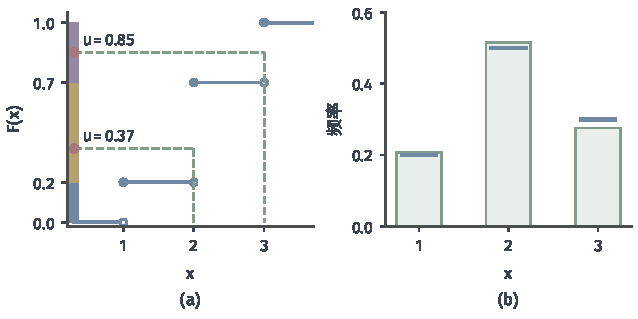
\includegraphics[width=108mm]{figures/07-probability/08-sampling-and-integration/matplotlib/sgen-discrete-inverse/figure.pdf}
  \caption{离散分布$p=(0.2,0.5,0.3)$的逆变换采样。(a)蓝线是分布函数，纵轴上的蓝、黄、紫三段是累计区间$(0,0.2]$、$(0.2,0.7]$、$(0.7,1]$；绿色虚线从$u=0.37$与$u=0.85$出发，分别落到$2$和$3$。(b)绿色柱是$1000$个样本（种子$11$）的频率$0.208,0.516,0.276$，蓝色短横线是真实概率。}
  \label{fig:sgen-discrete-inverse}
\end{BookInlineFigure}

式~\eqref{eq:sgen-discrete-inverse}的计算量在于找到$u$落在哪一段。从$k=1$起逐段比较，需要比较的次数是$X$对应的下标$k$，平均$\sum_kkp_k$次；例中为$0.2+1.0+0.9=2.1$次。若先把各值按概率从大到小排列，同一分布的平均次数降为$1\cdot0.5+2\cdot0.3+3\cdot0.2=1.7$次。$K$很大时，可以预先存好累计概率，用二分查找，每次约$\log_2K$次比较。

含原子的连续分布也由同一公式处理。分布函数在原子处的跳跃，对应$Q$的一段水平平台：长度等于原子概率的一段$u$全部被送到同一个点。第~\ref{chap:probability-spaces}章的等待时间在$0$处有概率$0.3$的原子，$u\le0.3$时输出$0$，就是这种情形。

\paragraph{需要数值反演的情形}
很多分布的$F$可以计算，$Q$却没有解析式。例如$\operatorname{Gamma}(2,1)$的分布函数是
\begin{equation}
  F(x)=1-(1+x)\mathrm{e}^{-x},\qquad x\ge0,
  \label{eq:sgen-gamma2-cdf}
\end{equation}
方程$F(x)=u$解不出初等的$x$。这时只能用数值方法近似求$Q(u)$。最稳妥的是二分法，它只用到$F$的单调性和式~\eqref{eq:sgen-quantile}的等价关系。

二分法的依据是：对任意点$m$，判断$F(m)\ge u$是否成立，就知道$Q(u)\le m$还是$Q(u)>m$。若已知$Q(u)$落在区间$(a,b]$中，取中点$m=(a+b)/2$做一次判断，就能把区间缩小一半，同时保持“$Q(u)$在区间内”这一事实。$k$轮后区间长度为$(b-a)/2^{k}$，输出中点，误差不超过区间长度的一半。

\needspace{6\baselineskip}
\paragraph{变量}
\begin{itemize}
  \item $u\in(0,1)$：基础随机数，整个过程中不变。
  \item $a<b$：当前区间的端点，始终满足$F(a)<u\le F(b)$，于是$Q(u)\in(a,b]$。
  \item $m$：当前区间的中点。
\end{itemize}

\paragraph{初始化}
取一个区间$(a,b]$，使$F(a)<u\le F(b)$。例中取$u=0.37$，$a=0$，$b=8$，因为
\[
  F(0)=0<0.37,\qquad F(8)=1-9\mathrm{e}^{-8}\approx0.9970\ge0.37 .
\]

\needspace{6\baselineskip}
\paragraph{每轮更新}
\begin{enumerate}
  \item \textbf{取中点。}令$m=(a+b)/2$，计算$F(m)$。例中第一轮$m=4$，由式~\eqref{eq:sgen-gamma2-cdf}，
  \[
    F(4)=1-5\mathrm{e}^{-4}\approx0.9084 .
  \]
  \item \textbf{缩小区间。}若$F(m)\ge u$，则$Q(u)\le m$，令$b\leftarrow m$；否则$Q(u)>m$，令$a\leftarrow m$。例中$0.9084\ge0.37$，区间变为$(0,4]$。

  以后各轮的中点、函数值和新区间依次为
  \[
    \begin{aligned}
      m&=2,& F(2)&\approx0.5940,& &(0,2];\\
      m&=1,& F(1)&\approx0.2642,& &(1,2];\\
      m&=1.5,& F(1.5)&\approx0.4422,& &(1,1.5];\\
      m&=1.25,& F(1.25)&\approx0.3554,& &(1.25,1.5].
    \end{aligned}
  \]
  \item \textbf{停止。}区间长度不超过预先给定的$2\delta$时停止，输出中点。例中取$\delta=0.125$，第五轮后长度为$0.25$，停止。
\end{enumerate}
最终输出$\widetilde{x}=1.375$。用更多轮次算出的真值是$Q(0.37)\approx1.2910$，误差约$0.084$，在$\delta=0.125$以内。图~\ref{fig:sgen-bisection-inverse}(a)画出了五个中点。

\paragraph{反演误差怎样改变输出分布}
数值反演输出的不是$Q(U)$，而是近似值$\widetilde{X}=\widetilde{Q}(U)$。它的分布已经不是$F$，问题是偏差多大。下面的引理把每个$u$上的反演误差转成分布函数的偏差。

\begin{lemma}[反演误差的传递]
\label{lem:sgen-inversion-error}
设$\delta\ge0$，函数$\widetilde{Q}$对一切$u\in(0,1)$满足$\lvert\widetilde{Q}(u)-Q(u)\rvert\le\delta$。记$\widetilde{F}$为$\widetilde{X}=\widetilde{Q}(U)$的分布函数，则对一切实数$x$，
\begin{equation}
  F(x-\delta)\le\widetilde{F}(x)\le F(x+\delta).
  \label{eq:sgen-inversion-band}
\end{equation}
若$F$还有不超过$L$的密度，则$\sup_x\lvert\widetilde{F}(x)-F(x)\rvert\le L\delta$。
\end{lemma}

\begin{proof}
若$\widetilde{X}\le x$，则$Q(U)\le\widetilde{X}+\delta\le x+\delta$，所以事件$\{\widetilde{X}\le x\}$包含于$\{Q(U)\le x+\delta\}$。取概率，由$Q(U)$的分布函数是$F$，得$\widetilde{F}(x)\le F(x+\delta)$。

反过来，若$Q(U)\le x-\delta$，则$\widetilde{X}\le Q(U)+\delta\le x$，所以$\{Q(U)\le x-\delta\}$包含于$\{\widetilde{X}\le x\}$，取概率得$F(x-\delta)\le\widetilde{F}(x)$。

若密度不超过$L$，则$F(x+\delta)-F(x)\le L\delta$，$F(x)-F(x-\delta)\le L\delta$，代入式~\eqref{eq:sgen-inversion-band}即得最后一句。
\end{proof}

引理的条件是“对所有$u$都有误差界$\delta$”，这一条在实际中容易被破坏。上面的二分法从固定区间$(0,8]$出发，当$u>F(8)\approx0.9970$时$Q(u)>8$，初始化条件不成立，二分法的每一轮都把区间推向右端，最终输出$7.875$，误差可以任意大。于是约$0.3\%$的尾部质量被搬到了$7.875$这一个点上。要保住误差界，初始化时须先把$b$向右扩大到$F(b)\ge u$为止。

即使误差界成立，输出的分布形状也可能改变。固定做五轮二分时，输出总是某个长$0.25$的小区间的中点，$\widetilde{X}$只取有限个值，是离散分布。图~\ref{fig:sgen-bisection-inverse}(b)画出它的分布函数：一条阶梯，夹在式~\eqref{eq:sgen-inversion-band}的两条紫色虚线之间。$\operatorname{Gamma}(2,1)$的密度$x\mathrm{e}^{-x}$的最大值是$\mathrm{e}^{-1}\approx0.368$，按引理，分布函数的偏差不超过$0.368\times0.125\approx0.046$；数值计算的最大偏差约为$0.0456$。用这样的样本估计依赖于细小尺度的量（例如落在某个短区间内的概率），偏差会比估计期望时明显。

\begin{BookInlineFigure}
  \centering
  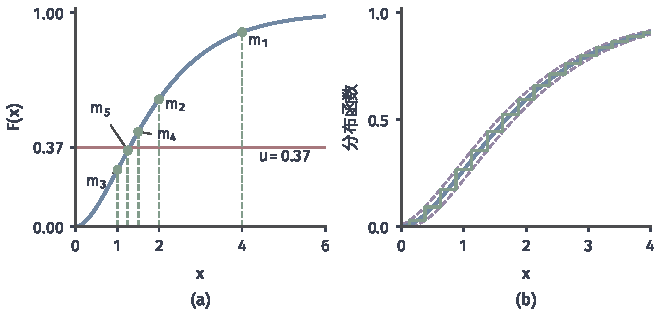
\includegraphics[width=112mm]{figures/07-probability/08-sampling-and-integration/matplotlib/sgen-bisection-inverse/figure.pdf}
  \caption{用二分法数值反演$\operatorname{Gamma}(2,1)$的分布函数。(a)蓝线是$F(x)=1-(1+x)\mathrm{e}^{-x}$，红线是$u=0.37$，绿点是五轮的中点$m_1,\dots,m_5=4,2,1,1.5,1.25$，最后区间为$(1.25,1.5]$。(b)固定做五轮时输出的分布函数（绿色阶梯）与$F$（蓝线），紫色虚线是$F(x-0.125)$与$F(x+0.125)$，阶梯始终夹在两者之间。}
  \label{fig:sgen-bisection-inverse}
\end{BookInlineFigure}

二分法每轮把误差减半，达到$\delta$需要约$\log_2((b-a)/\delta)$次分布函数求值。若$F$有可以计算的密度$f$，也可以用Newton迭代$x\leftarrow x-(F(x)-u)/f(x)$，在解附近每轮有效数字约翻一倍，但初值不好时可能越出定义域，常与二分法配合使用。不论用哪种方法，停止规则给出的误差界都要对全部$u$成立，引理~\ref{lem:sgen-inversion-error}才能用来估计输出分布的偏差。

\subsection{高斯样本生成}
\label{sec:sgen-gaussian}

高斯分布是最常用的目标，它的生成分两步：先生成独立的标准高斯坐标，再用一个仿射变换调出指定的均值与协方差。

\paragraph{独立标准高斯坐标}
标准高斯的分布函数$\Phi$连续且严格递增，由逆变换采样，$Z=\Phi^{-1}(U)$服从$\mathcal{N}(0,1)$。$\Phi^{-1}$没有初等表达式，常用的数值程序以有理函数逼近，在双精度下的误差已接近舍入误差，按引理~\ref{lem:sgen-inversion-error}，对输出分布的影响可以忽略。对$d$个相互独立的基础随机数分别作变换，
\[
  Z_j=\Phi^{-1}(U_j),\qquad j=1,\dots,d,
\]
各$Z_j$是不同基础随机数的函数，所以相互独立，组成的向量$\bm{Z}$服从$\mathcal{N}(\bm{0},\bm{I})$。式~\eqref{eq:sgen-box-muller}是另一种办法，每两个基础随机数给出两个独立的标准高斯数，只用到对数与三角函数。

例如取$u_1=0.37$、$u_2=0.80$，
\[
  z_1=\Phi^{-1}(0.37)\approx-0.3319,\qquad z_2=\Phi^{-1}(0.80)\approx0.8416 .
\]

\paragraph{仿射变换}
要生成$\mathcal{N}(\bm{\mu},\bm{\Sigma})$，其中$\bm{\mu}\in\mathbb{R}^{d}$是均值向量，$\bm{\Sigma}\in\mathbb{R}^{d\times d}$是对称半正定的协方差矩阵，先把$\bm{\Sigma}$分解为
\begin{equation}
  \bm{\Sigma}=\bm{A}\bm{A}^{\top},\qquad \bm{A}\in\mathbb{R}^{d\times r},
  \label{eq:sgen-cov-factor}
\end{equation}
再取$r$个独立标准高斯坐标组成$\bm{Z}$，令
\begin{equation}
  \bm{X}=\bm{\mu}+\bm{A}\bm{Z}.
  \label{eq:sgen-gaussian-affine}
\end{equation}
由期望的线性，$\mathbb{E}[\bm{X}]=\bm{\mu}$；由协方差在线性变换下的规则，
\[
  \operatorname{Cov}(\bm{X})=\bm{A}\operatorname{Cov}(\bm{Z})\bm{A}^{\top}=\bm{A}\bm{I}\bm{A}^{\top}=\bm{\Sigma}.
\]
第~\ref{chap:multivariate-distributions}章正是用这种形式定义多元高斯分布的，并证明了$\bm{\mu}+\bm{A}\bm{Z}$的分布只依赖于$\bm{A}\bm{A}^{\top}$，所以不论选哪个因子，都有$\bm{X}\sim\mathcal{N}(\bm{\mu},\bm{\Sigma})$。这一论证没有用到密度，因而不要求$\bm{\Sigma}$可逆。

因子$\bm{A}$有两种常用取法。$\bm{\Sigma}$正定时，Cholesky分解给出对角元为正的下三角矩阵$\bm{L}$，使$\bm{\Sigma}=\bm{L}\bm{L}^{\top}$，计算量约为$d^{3}/3$次乘法（可参考\BookChapterRef{chap:direct-linear-solvers}{卷二第12章“线性方程的直接求解”}）。$\bm{\Sigma}$只是半正定时，Cholesky分解会遇到零主元，可改用谱分解$\bm{\Sigma}=\bm{V}\bm{\Lambda}\bm{V}^{\top}$（可参考\BookChapterRef{chap:eigen-spectral-decomposition}{卷二第6章“谱分解”}），取$\bm{A}=\bm{V}\bm{\Lambda}^{1/2}$，并去掉特征值为零的列。分解只需做一次，之后每个样本只需$d$个标准高斯数和一次矩阵乘向量。

用一个二维例子走一遍。取
\[
  \bm{\mu}=\begin{bmatrix}1\\0\end{bmatrix},\qquad
  \bm{\Sigma}=\begin{bmatrix}4&2\\2&2\end{bmatrix},\qquad
  \bm{L}=\begin{bmatrix}2&0\\1&1\end{bmatrix},
\]
可以直接验证$\bm{L}\bm{L}^{\top}=\bm{\Sigma}$。代入上面的$z_1,z_2$，由式~\eqref{eq:sgen-gaussian-affine}，
\[
  \bm{x}=\begin{bmatrix}1+2z_1\\ z_1+z_2\end{bmatrix}\approx\begin{bmatrix}0.3363\\0.5098\end{bmatrix}.
\]
下三角结构使第一个坐标只用到$z_1$，第二个坐标用到$z_1$和$z_2$；两个坐标共用$z_1$，这正是它们的协方差$2$的来源。

\paragraph{奇异协方差}
若$\bm{\Sigma}$的秩$r<d$，式~\eqref{eq:sgen-gaussian-affine}仍然给出正确的分布，但$\bm{X}-\bm{\mu}=\bm{A}\bm{Z}$总落在$\bm{A}$的列空间中，这是一个$r$维子空间。例如
\[
  \bm{\Sigma}=\begin{bmatrix}1&2\\2&4\end{bmatrix}=\bm{a}\bm{a}^{\top},\qquad \bm{a}=\begin{bmatrix}1\\2\end{bmatrix},
\]
只需一个标准高斯数，$\bm{X}=\bm{\mu}+Z_1\bm{a}$全部落在过$\bm{\mu}$、方向为$\bm{a}$的直线上。这条直线在平面上的面积为零，$\bm{X}$在$\mathbb{R}^{2}$中没有密度，式~\eqref{eq:sgen-change-of-variables}无从使用；推前的论证不受影响。图~\ref{fig:sgen-gaussian-affine}对比了三种情形。

\begin{BookInlineFigure}
  \centering
  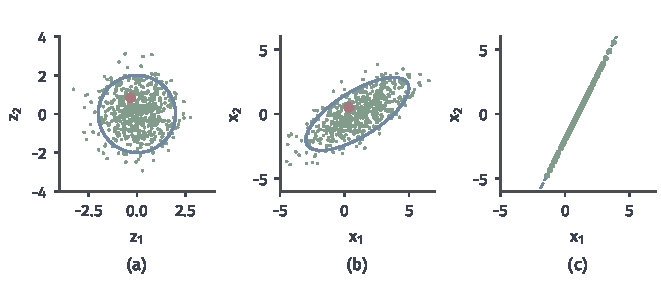
\includegraphics[width=112mm]{figures/07-probability/08-sampling-and-integration/matplotlib/sgen-gaussian-affine/figure.pdf}
  \caption{由独立标准高斯坐标生成指定协方差的高斯样本，$600$个样本（种子$5$）。(a)标准高斯$\bm{Z}$，蓝线是半径$2$的圆，红点是$(\Phi^{-1}(0.37),\Phi^{-1}(0.80))$；(b)$\bm{X}=\bm{\mu}+\bm{L}\bm{Z}$，$\bm{\mu}=(1,0)^{\top}$，$\bm{\Sigma}=\bm{L}\bm{L}^{\top}$，圆被变成椭圆，红点是例中的$(0.336,0.510)$；(c)秩为$1$的$\bm{\Sigma}=\bm{a}\bm{a}^{\top}$，样本全部落在蓝色虚线上。}
  \label{fig:sgen-gaussian-affine}
\end{BookInlineFigure}

奇异协方差在数值上还有一个隐患。若$\bm{\Sigma}$本应奇异，由于舍入它的最小特征值可能算成很小的负数，Cholesky分解随之失败；若$\bm{\Sigma}$本应正定但极接近奇异，分解得到的因子误差也会很大。谱分解可以把很小的负特征值截为零，但截断改变了协方差，偏差的大小应与$\bm{\Sigma}$的元素尺度一起报告。
